%
% einleitung.tex -- Beispiel-File für die Einleitung
%
% (c) 2020 Prof Dr Andreas Müller, Hochschule Rapperswil
%
\section{Einleitung\label{legendre:section:einleitung}}
\rhead{Einleitung}
Die {\em zugeordneten Legendrepolynome} (engl. {\em associated Legendre polynomials}) $P^m_l$ besitzen zwei Parameter, $m$ und $l$.
Mittels diesen beiden Parameter lassen sich einige Rekursionsbeziehungen (engl. {\em recurrence relation}) aufstellen.
Zur Berechnung der Werte von zugeordneten Legendrepolynomen wird normalerweise auf eine solche Rekursionsbeziehung zurückgegriffen.
Die Rekursionsbeziehungen werden bevorzugt, da deren Alternativen Nachteile mit sich bringen.
So ist beispielsweise die Verwendung der geschlossenen Form
\begin{equation}
P^{m}_{l}(x)
=
(-1)^m \cdot 2^l \cdot (1-x^2)^{m/2}
\cdot \sum_{k=m}^{l} \frac{k!}{(k-m)!} \cdot x^{k-m}
\cdot \binom{l}{m} \binom{\frac{l+k-1}{2}}{l}
\label{legendre:geschlosseneform}
\end{equation}
für ein zugeordnetes Legendrepolynom $P^m_l$ rechnerisch zu aufwendig.
Andererseits ist es möglich, die Polynomfunktionen für die verschiedenen Werte von $l$ und $m$ aufzustellen.
Dies ist jedoch für höhere zugeordnete Legedrepolynome nicht praktikabel.

Von den Rekursionsbeziehungen gibt es eine ganze Liste voll und es ist gut möglich, dass nicht alle davon numerisch stabil sind.
Es ist daher möglich, dass bei einer unglücklichen Wahl einer solchen Rekursionsbeziehung numerische Probleme auftreten können, die zu völlig falschen Resultaten führen.
Dass ein solches numerisches Problem auftreten kann, wird leider oft vergessen.
Zusätzlich ist es eine anspruchsvolle Aufgabe, solche numerischen Instabilitäten vorzeitig zu erkennen.
Aus diesen Gründen ist es nicht verwunderlich, dass sogar namhafte Bibliotheken numerisch instabile Implementationen enthalten.
So ist beispielsweise die Implementation der zugeordneten Legendrepolynome auf Wolfram Alpha \cite{legendre:wolfram-alpha} numerisch nicht stabil, wie gut in der Abbildung \ref{legendre:fig:wolframalpha} zu sehen ist.
Aus diesen Gründen befasst sich dieses Kapitel mit der Stabilität oder eben Instabilität der Rekursionsbeziehungen für zugeordnete Legendrepolynome.

\begin{figure}[!ht]
\centering
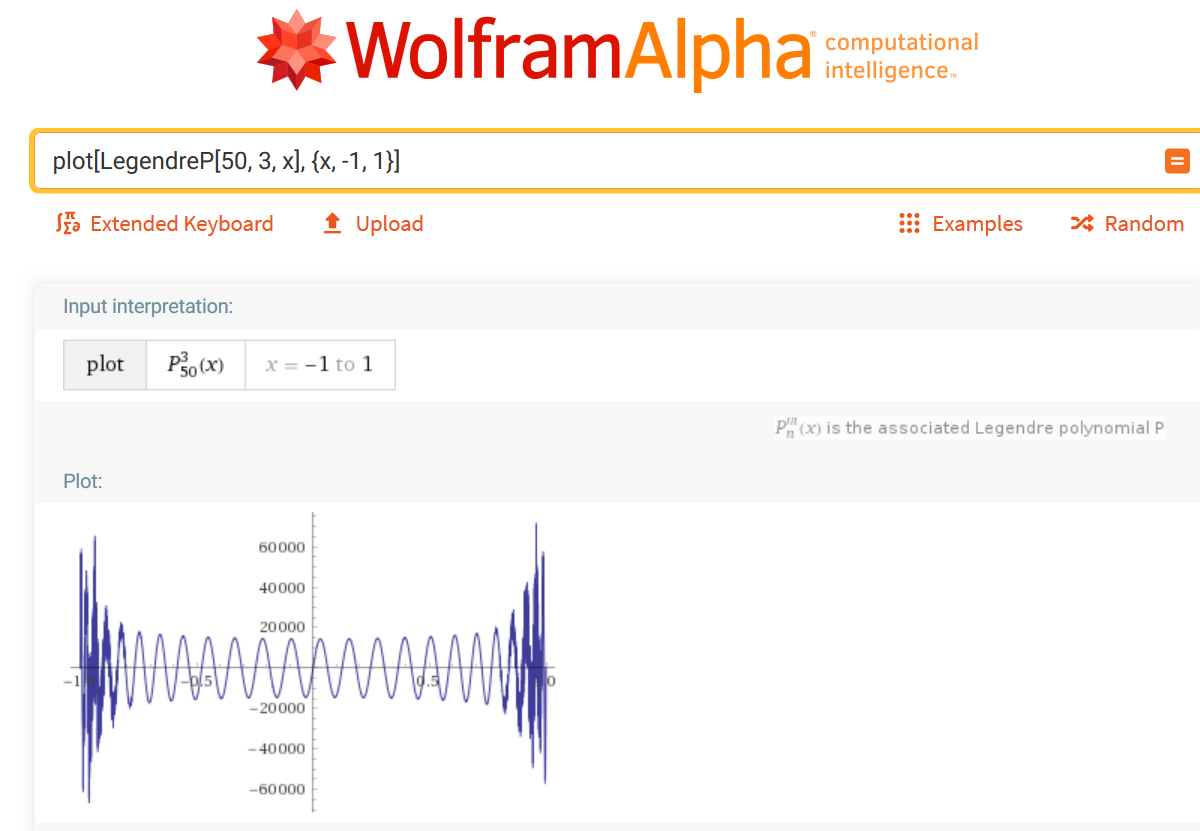
\includegraphics[width=0.9\linewidth]{papers/legendre/plots/wolframalpha}
\caption{Von Wolram Alpha \cite{legendre:wolfram-alpha} generierter Graph des zugeordneten Legendrepolynoms mit \texorpdfstring{$l=50$}{l=50} und \texorpdfstring{$m=3$}{m=3}. Deutliche numerische Instabilitäten nahe den Randbereichen.}
\label{legendre:fig:wolframalpha}
\end{figure}
